\PassOptionsToPackage{unicode=true}{hyperref} % options for packages loaded elsewhere
\PassOptionsToPackage{hyphens}{url}
%
\documentclass[ignorenonframetext,]{beamer}
\usepackage{pgfpages}
\setbeamertemplate{caption}[numbered]
\setbeamertemplate{caption label separator}{: }
\setbeamercolor{caption name}{fg=normal text.fg}
\beamertemplatenavigationsymbolsempty
% Prevent slide breaks in the middle of a paragraph:
\widowpenalties 1 10000
\raggedbottom
\setbeamertemplate{part page}{
\centering
\begin{beamercolorbox}[sep=16pt,center]{part title}
  \usebeamerfont{part title}\insertpart\par
\end{beamercolorbox}
}
\setbeamertemplate{section page}{
\centering
\begin{beamercolorbox}[sep=12pt,center]{part title}
  \usebeamerfont{section title}\insertsection\par
\end{beamercolorbox}
}
\setbeamertemplate{subsection page}{
\centering
\begin{beamercolorbox}[sep=8pt,center]{part title}
  \usebeamerfont{subsection title}\insertsubsection\par
\end{beamercolorbox}
}
\AtBeginPart{
  \frame{\partpage}
}
\AtBeginSection{
  \ifbibliography
  \else
    \frame{\sectionpage}
  \fi
}
\AtBeginSubsection{
  \frame{\subsectionpage}
}
\usepackage{lmodern}
\usepackage{amssymb,amsmath}
\usepackage{ifxetex,ifluatex}
\usepackage{fixltx2e} % provides \textsubscript
\ifnum 0\ifxetex 1\fi\ifluatex 1\fi=0 % if pdftex
  \usepackage[T1]{fontenc}
  \usepackage[utf8]{inputenc}
  \usepackage{textcomp} % provides euro and other symbols
\else % if luatex or xelatex
  \usepackage{unicode-math}
  \defaultfontfeatures{Ligatures=TeX,Scale=MatchLowercase}
\fi
% use upquote if available, for straight quotes in verbatim environments
\IfFileExists{upquote.sty}{\usepackage{upquote}}{}
% use microtype if available
\IfFileExists{microtype.sty}{%
\usepackage[]{microtype}
\UseMicrotypeSet[protrusion]{basicmath} % disable protrusion for tt fonts
}{}
\IfFileExists{parskip.sty}{%
\usepackage{parskip}
}{% else
\setlength{\parindent}{0pt}
\setlength{\parskip}{6pt plus 2pt minus 1pt}
}
\usepackage{hyperref}
\hypersetup{
            pdftitle={Data Science, Séance 7 : Visualisation avec ggplot},
            pdfauthor={Etienne Côme},
            pdfborder={0 0 0},
            breaklinks=true}
\urlstyle{same}  % don't use monospace font for urls
\newif\ifbibliography
\usepackage{color}
\usepackage{fancyvrb}
\newcommand{\VerbBar}{|}
\newcommand{\VERB}{\Verb[commandchars=\\\{\}]}
\DefineVerbatimEnvironment{Highlighting}{Verbatim}{commandchars=\\\{\}}
% Add ',fontsize=\small' for more characters per line
\usepackage{framed}
\definecolor{shadecolor}{RGB}{248,248,248}
\newenvironment{Shaded}{\begin{snugshade}}{\end{snugshade}}
\newcommand{\AlertTok}[1]{\textcolor[rgb]{0.94,0.16,0.16}{#1}}
\newcommand{\AnnotationTok}[1]{\textcolor[rgb]{0.56,0.35,0.01}{\textbf{\textit{#1}}}}
\newcommand{\AttributeTok}[1]{\textcolor[rgb]{0.77,0.63,0.00}{#1}}
\newcommand{\BaseNTok}[1]{\textcolor[rgb]{0.00,0.00,0.81}{#1}}
\newcommand{\BuiltInTok}[1]{#1}
\newcommand{\CharTok}[1]{\textcolor[rgb]{0.31,0.60,0.02}{#1}}
\newcommand{\CommentTok}[1]{\textcolor[rgb]{0.56,0.35,0.01}{\textit{#1}}}
\newcommand{\CommentVarTok}[1]{\textcolor[rgb]{0.56,0.35,0.01}{\textbf{\textit{#1}}}}
\newcommand{\ConstantTok}[1]{\textcolor[rgb]{0.00,0.00,0.00}{#1}}
\newcommand{\ControlFlowTok}[1]{\textcolor[rgb]{0.13,0.29,0.53}{\textbf{#1}}}
\newcommand{\DataTypeTok}[1]{\textcolor[rgb]{0.13,0.29,0.53}{#1}}
\newcommand{\DecValTok}[1]{\textcolor[rgb]{0.00,0.00,0.81}{#1}}
\newcommand{\DocumentationTok}[1]{\textcolor[rgb]{0.56,0.35,0.01}{\textbf{\textit{#1}}}}
\newcommand{\ErrorTok}[1]{\textcolor[rgb]{0.64,0.00,0.00}{\textbf{#1}}}
\newcommand{\ExtensionTok}[1]{#1}
\newcommand{\FloatTok}[1]{\textcolor[rgb]{0.00,0.00,0.81}{#1}}
\newcommand{\FunctionTok}[1]{\textcolor[rgb]{0.00,0.00,0.00}{#1}}
\newcommand{\ImportTok}[1]{#1}
\newcommand{\InformationTok}[1]{\textcolor[rgb]{0.56,0.35,0.01}{\textbf{\textit{#1}}}}
\newcommand{\KeywordTok}[1]{\textcolor[rgb]{0.13,0.29,0.53}{\textbf{#1}}}
\newcommand{\NormalTok}[1]{#1}
\newcommand{\OperatorTok}[1]{\textcolor[rgb]{0.81,0.36,0.00}{\textbf{#1}}}
\newcommand{\OtherTok}[1]{\textcolor[rgb]{0.56,0.35,0.01}{#1}}
\newcommand{\PreprocessorTok}[1]{\textcolor[rgb]{0.56,0.35,0.01}{\textit{#1}}}
\newcommand{\RegionMarkerTok}[1]{#1}
\newcommand{\SpecialCharTok}[1]{\textcolor[rgb]{0.00,0.00,0.00}{#1}}
\newcommand{\SpecialStringTok}[1]{\textcolor[rgb]{0.31,0.60,0.02}{#1}}
\newcommand{\StringTok}[1]{\textcolor[rgb]{0.31,0.60,0.02}{#1}}
\newcommand{\VariableTok}[1]{\textcolor[rgb]{0.00,0.00,0.00}{#1}}
\newcommand{\VerbatimStringTok}[1]{\textcolor[rgb]{0.31,0.60,0.02}{#1}}
\newcommand{\WarningTok}[1]{\textcolor[rgb]{0.56,0.35,0.01}{\textbf{\textit{#1}}}}
\usepackage{longtable,booktabs}
\usepackage{caption}
% These lines are needed to make table captions work with longtable:
\makeatletter
\def\fnum@table{\tablename~\thetable}
\makeatother
\usepackage{graphicx,grffile}
\makeatletter
\def\maxwidth{\ifdim\Gin@nat@width>\linewidth\linewidth\else\Gin@nat@width\fi}
\def\maxheight{\ifdim\Gin@nat@height>\textheight\textheight\else\Gin@nat@height\fi}
\makeatother
% Scale images if necessary, so that they will not overflow the page
% margins by default, and it is still possible to overwrite the defaults
% using explicit options in \includegraphics[width, height, ...]{}
\setkeys{Gin}{width=\maxwidth,height=\maxheight,keepaspectratio}
\setlength{\emergencystretch}{3em}  % prevent overfull lines
\providecommand{\tightlist}{%
  \setlength{\itemsep}{0pt}\setlength{\parskip}{0pt}}
\setcounter{secnumdepth}{0}

% set default figure placement to htbp
\makeatletter
\def\fps@figure{htbp}
\makeatother


\title{Data Science, Séance 7 : Visualisation avec ggplot}
\author{Etienne Côme}
\date{21 novembre 2018}

\begin{document}
\frame{\titlepage}

\begin{frame}{Visualisation ?}
\protect\hypertarget{visualisation}{}

``Transformation of the symbolic into the geometric'' {[}McCormick et
al.~1987{]}

``\ldots{} finding the artificial memory that best supports our natural
means of perception.'' {[}Bertin 1967{]}

``The use of computer-generated, interactive, visual representations of
data to amplify cognition.'' {[}Card, Mackinlay, \& Shneiderman 1999{]}

\end{frame}

\begin{frame}{Pourquoi visualiser ?}
\protect\hypertarget{pourquoi-visualiser}{}

\begin{block}{Intégrer l'humain dans la boucle}

Répondre a des questions ou trouver des questions ?

Prendre des décisions

Remettre les données dans leur contexte

Amplifier la mémoire

Calcul graphique

Trouver des schémas, des patterns

Présenter des arguments

Inspirer

\end{block}

\end{frame}

\begin{frame}{Pourquoi visualiser ?}
\protect\hypertarget{pourquoi-visualiser-1}{}

\begin{block}{Analyser :}

Développer et critiquer des hypothèses

Découvrir des erreurs

Trouver des patterns

\end{block}

\begin{block}{Communiquer}

Partager et convaincre

Collaborer et réviser

\#\#{Anscombe quartet}

\begin{longtable}[]{@{}rrrrr@{}}
\toprule
g & mean\_x & mean\_y & sd\_x & sd\_y\tabularnewline
\midrule
\endhead
1 & 9 & 7.500909 & 3.316625 & 2.031568\tabularnewline
2 & 9 & 7.500909 & 3.316625 & 2.031657\tabularnewline
3 & 9 & 7.500000 & 3.316625 & 2.030424\tabularnewline
4 & 9 & 7.500909 & 3.316625 & 2.030578\tabularnewline
\bottomrule
\end{longtable}

\#\#{Anscombe quartet} \{data-background=\#ffffff\}
\includegraphics{Seance7_files/figure-beamer/unnamed-chunk-2-1.pdf}

\end{block}

\end{frame}

\begin{frame}{Cholera map (John Snow)}
\protect\hypertarget{cholera-map-john-snow}{}

\end{frame}

\begin{frame}{}
\protect\hypertarget{section}{}

{ Visualiser }

=

encoder dans des

{ variables graphiques}

les données

\end{frame}

\begin{frame}{{Variables graphiques}}
\protect\hypertarget{variables-graphiques}{}

Bertin Jacques, Sémiologie graphique, Paris, Mouton/Gauthier-Villars,
1967.

\end{frame}

\begin{frame}{{Variables graphiques}}
\protect\hypertarget{variables-graphiques-1}{}

Bertin Jacques, Sémiologie graphique, Paris, Mouton/Gauthier-Villars,
1967.

\end{frame}

\begin{frame}{Marques // variables graphiques}
\protect\hypertarget{marques-variables-graphiques}{}

\begin{block}{Marques :}

Eléments de base du graphiques

\end{block}

\begin{block}{Variables graphique (chanels) :}

Ce qui va varier en fonctions des données

\end{block}

\end{frame}

\begin{frame}{{Variables graphiques, marques }}
\protect\hypertarget{variables-graphiques-marques}{}

\end{frame}

\begin{frame}{{Variables graphiques, marques }}
\protect\hypertarget{variables-graphiques-marques-1}{}

Toutes les variables graphiques ne se valent pas.

\end{frame}

\begin{frame}{{Variables graphiques, marques }}
\protect\hypertarget{variables-graphiques-marques-2}{}

{Choisir une variable graphique adapté aux type de la variable
représenté}

\end{frame}

\begin{frame}{{Variables graphiques, marques }}
\protect\hypertarget{variables-graphiques-marques-3}{}

Ce qui est intéressant n'est pas toujours ce que l'on a au départ.

\end{frame}

\begin{frame}{pré-attentive processing}
\protect\hypertarget{pruxe9-attentive-processing}{}

\begin{block}{Combien de 3 ?}

1281768756138976546984506985604982826762
9809858458224509856458945098450980943585
9091030209905959595772564675050678904567
8845789809821677654876364908560912949686

\end{block}

\end{frame}

\begin{frame}{pré-attentive processing}
\protect\hypertarget{pruxe9-attentive-processing-1}{}

\begin{block}{Combien de 3 ?}

12817687561{3}8976546984506985604982826762
980985845822450985645894509845098094{3}585
90910{3}0209905959595772564675050678904567
8845789809821677654876{3}64908560912949686

\end{block}

\end{frame}

\begin{frame}{{pré-attentive processing}}
\protect\hypertarget{pruxe9-attentive-processing-2}{}

\end{frame}

\begin{frame}{{pré-attentive processing}}
\protect\hypertarget{pruxe9-attentive-processing-3}{}

\end{frame}

\begin{frame}{{pré-attentive processing}}
\protect\hypertarget{pruxe9-attentive-processing-4}{}

\end{frame}

\begin{frame}{}
\protect\hypertarget{section-1}{}

\end{frame}

\begin{frame}{}
\protect\hypertarget{section-2}{}

\end{frame}

\begin{frame}{}
\protect\hypertarget{section-3}{}

\end{frame}

\begin{frame}[fragile]{}
\protect\hypertarget{section-4}{}

\begin{Shaded}
\begin{Highlighting}[]
\KeywordTok{library}\NormalTok{(ggplot2)}
\KeywordTok{ggplot}\NormalTok{(mpg)}\OperatorTok{+}\KeywordTok{geom_point}\NormalTok{(}\KeywordTok{aes}\NormalTok{(}\DataTypeTok{x=}\NormalTok{cty,}\DataTypeTok{y=}\NormalTok{hwy,}\DataTypeTok{color=}\NormalTok{class))}
\end{Highlighting}
\end{Shaded}

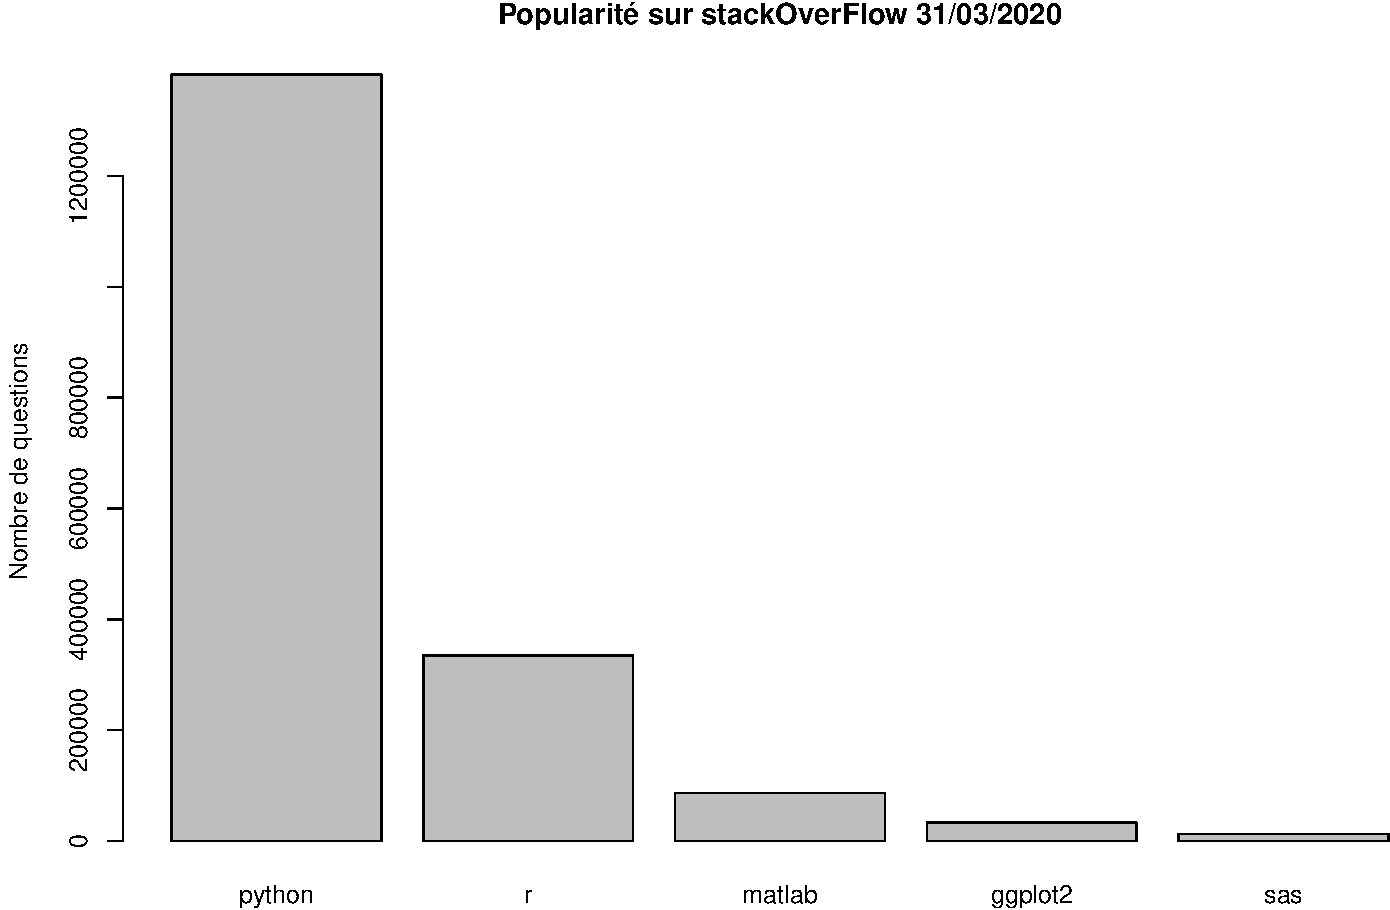
\includegraphics{Seance7_files/figure-beamer/unnamed-chunk-3-1.pdf}

\end{frame}

\begin{frame}{}
\protect\hypertarget{section-5}{}

Questions ? type des variables ?

{continues ?} {discrètes ?} {ordonnées ?} {temporelles ?} {spatiales ?}

\end{frame}

\begin{frame}{}
\protect\hypertarget{section-6}{}

{Des catégories}

et

{ une quantité pour chaque catégorie}

\end{frame}

\begin{frame}{}
\protect\hypertarget{section-7}{}

le bar chart

\end{frame}

\begin{frame}[fragile]{{ le bar chart}}
\protect\hypertarget{le-bar-chart}{}

\begin{Shaded}
\begin{Highlighting}[]
\KeywordTok{library}\NormalTok{(rjson)}
\KeywordTok{library}\NormalTok{(dplyr)}
\NormalTok{?mpg}
\end{Highlighting}
\end{Shaded}

dataset mpg

manufacturer.

model.

displ. engine displacement, in litres

\ldots{}

\end{frame}

\begin{frame}[fragile]{{ le bar chart}}
\protect\hypertarget{le-bar-chart-1}{}

\begin{Shaded}
\begin{Highlighting}[]
\NormalTok{m_cty =}\StringTok{ }\NormalTok{mpg }\OperatorTok\StringTok{ }\KeywordTok{group_by}\NormalTok{(manufacturer) }\OperatorTok\StringTok{ }\KeywordTok{summarize}\NormalTok{(}\DataTypeTok{mcty=}\KeywordTok{mean}\NormalTok{(cty))}
\KeywordTok{ggplot}\NormalTok{(}\DataTypeTok{data=}\NormalTok{m_cty)}\OperatorTok{+}
\StringTok{  }\KeywordTok{geom_bar}\NormalTok{(}\KeywordTok{aes}\NormalTok{(}\DataTypeTok{x=}\NormalTok{manufacturer,}\DataTypeTok{y=}\NormalTok{mcty),}\DataTypeTok{stat =} \StringTok{'identity'}\NormalTok{)}\OperatorTok{+}
\StringTok{  }\KeywordTok{scale_x_discrete}\NormalTok{(}\StringTok{"Manufacturer"}\NormalTok{)}\OperatorTok{+}
\StringTok{  }\KeywordTok{scale_y_continuous}\NormalTok{(}\StringTok{"Miles / Gallon (City conditions)"}\NormalTok{)}
\end{Highlighting}
\end{Shaded}

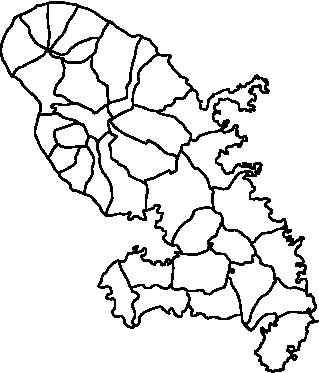
\includegraphics{Seance7_files/figure-beamer/unnamed-chunk-5-1.pdf}

\end{frame}

\begin{frame}[fragile]{{ Ordre ?}}
\protect\hypertarget{ordre}{}

\begin{Shaded}
\begin{Highlighting}[]
\NormalTok{m_cty_ordered =}\StringTok{ }\NormalTok{m_cty }\OperatorTok\StringTok{ }\KeywordTok{arrange}\NormalTok{(}\KeywordTok{desc}\NormalTok{(mcty)) }\OperatorTok\StringTok{ }
\StringTok{  }\KeywordTok{mutate}\NormalTok{(}\DataTypeTok{manufacturer=}\KeywordTok{factor}\NormalTok{(manufacturer,}\DataTypeTok{levels=}\NormalTok{manufacturer))}
\KeywordTok{ggplot}\NormalTok{(}\DataTypeTok{data=}\NormalTok{m_cty_ordered)}\OperatorTok{+}
\StringTok{  }\KeywordTok{geom_bar}\NormalTok{(}\KeywordTok{aes}\NormalTok{(}\DataTypeTok{x=}\NormalTok{manufacturer,}\DataTypeTok{y=}\NormalTok{mcty),}\DataTypeTok{stat =} \StringTok{'identity'}\NormalTok{)}\OperatorTok{+}
\StringTok{  }\KeywordTok{scale_x_discrete}\NormalTok{(}\StringTok{"Manufacturer"}\NormalTok{)}\OperatorTok{+}
\StringTok{  }\KeywordTok{scale_y_continuous}\NormalTok{(}\StringTok{"Miles / Gallon (City conditions)"}\NormalTok{)}
\end{Highlighting}
\end{Shaded}

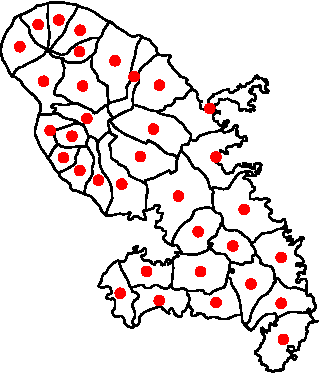
\includegraphics{Seance7_files/figure-beamer/unnamed-chunk-6-1.pdf}

\end{frame}

\begin{frame}[fragile]{{ Horizontal ?}}
\protect\hypertarget{horizontal}{}

\begin{Shaded}
\begin{Highlighting}[]
\KeywordTok{ggplot}\NormalTok{(}\DataTypeTok{data=}\NormalTok{m_cty_ordered)}\OperatorTok{+}
\StringTok{  }\KeywordTok{geom_bar}\NormalTok{(}\KeywordTok{aes}\NormalTok{(}\DataTypeTok{x=}\NormalTok{manufacturer,}\DataTypeTok{y=}\NormalTok{mcty),}\DataTypeTok{stat =} \StringTok{'identity'}\NormalTok{)}\OperatorTok{+}
\StringTok{  }\KeywordTok{scale_x_discrete}\NormalTok{(}\StringTok{"Manufacturer"}\NormalTok{)}\OperatorTok{+}
\StringTok{  }\KeywordTok{scale_y_continuous}\NormalTok{(}\StringTok{"Miles / Gallon (City conditions)"}\NormalTok{)}\OperatorTok{+}
\StringTok{  }\KeywordTok{coord_flip}\NormalTok{()}
\end{Highlighting}
\end{Shaded}

\includegraphics{Seance7_files/figure-beamer/unnamed-chunk-7-1.pdf}

\end{frame}

\begin{frame}{}
\protect\hypertarget{section-8}{}

La ligne :

{ 1 variable numérique}

en fonction du

{ temps}

\end{frame}

\begin{frame}[fragile]{}
\protect\hypertarget{section-9}{}

Données Vélib' aggrégées :

\begin{Shaded}
\begin{Highlighting}[]
\NormalTok{url=}\StringTok{"http://vlsstats.ifsttar.fr/data/temporalstats_Velib2018.json"}
\CommentTok{# lecture des données}
\NormalTok{data=}\KeywordTok{fromJSON}\NormalTok{(}\DataTypeTok{file=}\NormalTok{url)}
\CommentTok{# construction d'une liste de data.frame homogènes}
\NormalTok{tempstats.list=}\KeywordTok{lapply}\NormalTok{(data,}\ControlFlowTok{function}\NormalTok{(x)\{}
  \KeywordTok{data.frame}\NormalTok{(}\DataTypeTok{time=}\NormalTok{x}\OperatorTok{$}\StringTok{'_id'}\NormalTok{,}\DataTypeTok{nbbikes=}\NormalTok{x}\OperatorTok{$}\NormalTok{value}\OperatorTok{$}\NormalTok{total_available_bikes)\})}
\CommentTok{# concatenations des data.frame ?do.call}
\NormalTok{tempstats.df=}\KeywordTok{do.call}\NormalTok{(rbind,tempstats.list)}
\end{Highlighting}
\end{Shaded}

\end{frame}

\begin{frame}[fragile]{Ordre naturel imposé par le temps}
\protect\hypertarget{ordre-naturel-imposuxe9-par-le-temps}{}

\begin{Shaded}
\begin{Highlighting}[]
\KeywordTok{ggplot}\NormalTok{(}\DataTypeTok{data=}\NormalTok{tempstats.df,}\KeywordTok{aes}\NormalTok{(}\DataTypeTok{x=}\NormalTok{time,}\DataTypeTok{y=}\NormalTok{nbbikes))}\OperatorTok{+}\KeywordTok{geom_point}\NormalTok{()}
\end{Highlighting}
\end{Shaded}

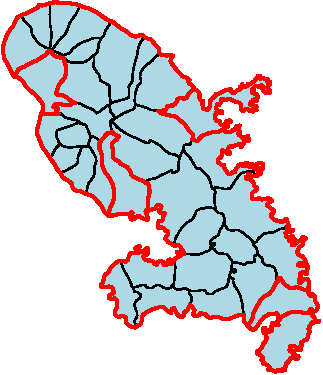
\includegraphics{Seance7_files/figure-beamer/unnamed-chunk-9-1.pdf}

\end{frame}

\begin{frame}[fragile]{Ordre naturel imposé par le temps}
\protect\hypertarget{ordre-naturel-imposuxe9-par-le-temps-1}{}

\begin{Shaded}
\begin{Highlighting}[]
\KeywordTok{ggplot}\NormalTok{(}\DataTypeTok{data=}\NormalTok{tempstats.df,}\KeywordTok{aes}\NormalTok{(}\DataTypeTok{x=}\NormalTok{time,}\DataTypeTok{y=}\NormalTok{nbbikes))}\OperatorTok{+}\KeywordTok{geom_line}\NormalTok{()}
\end{Highlighting}
\end{Shaded}

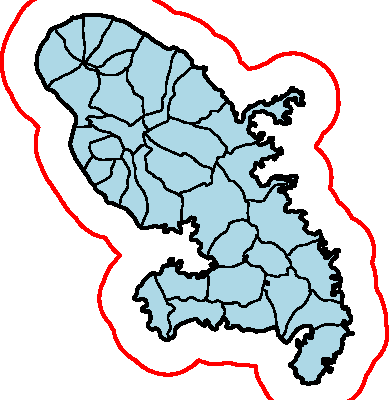
\includegraphics{Seance7_files/figure-beamer/unnamed-chunk-10-1.pdf}

\end{frame}

\begin{frame}[fragile]{Aspect ratio}
\protect\hypertarget{aspect-ratio}{}

\begin{Shaded}
\begin{Highlighting}[]
\KeywordTok{ggplot}\NormalTok{(}\DataTypeTok{data=}\NormalTok{tempstats.df,}\KeywordTok{aes}\NormalTok{(}\DataTypeTok{x=}\NormalTok{time,}\DataTypeTok{y=}\NormalTok{nbbikes))}\OperatorTok{+}\KeywordTok{geom_line}\NormalTok{()}
\end{Highlighting}
\end{Shaded}

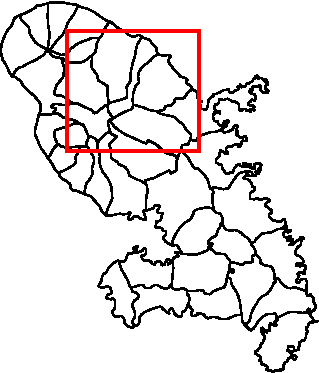
\includegraphics{Seance7_files/figure-beamer/unnamed-chunk-11-1.pdf}

\end{frame}

\begin{frame}[fragile]{Aspect ratio}
\protect\hypertarget{aspect-ratio-1}{}

\begin{Shaded}
\begin{Highlighting}[]
\KeywordTok{ggplot}\NormalTok{(}\DataTypeTok{data=}\NormalTok{tempstats.df,}\KeywordTok{aes}\NormalTok{(}\DataTypeTok{x=}\NormalTok{time,}\DataTypeTok{y=}\NormalTok{nbbikes))}\OperatorTok{+}\KeywordTok{geom_line}\NormalTok{()}
\end{Highlighting}
\end{Shaded}

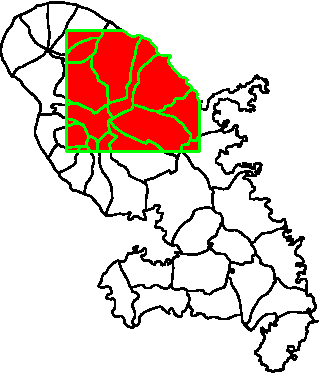
\includegraphics{Seance7_files/figure-beamer/unnamed-chunk-12-1.pdf}

\end{frame}

\begin{frame}[fragile]{Aspect ratio}
\protect\hypertarget{aspect-ratio-2}{}

\begin{Shaded}
\begin{Highlighting}[]
\KeywordTok{ggplot}\NormalTok{(}\DataTypeTok{data=}\NormalTok{tempstats.df,}\KeywordTok{aes}\NormalTok{(}\DataTypeTok{x=}\NormalTok{time,}\DataTypeTok{y=}\NormalTok{nbbikes))}\OperatorTok{+}\KeywordTok{geom_line}\NormalTok{()}
\end{Highlighting}
\end{Shaded}

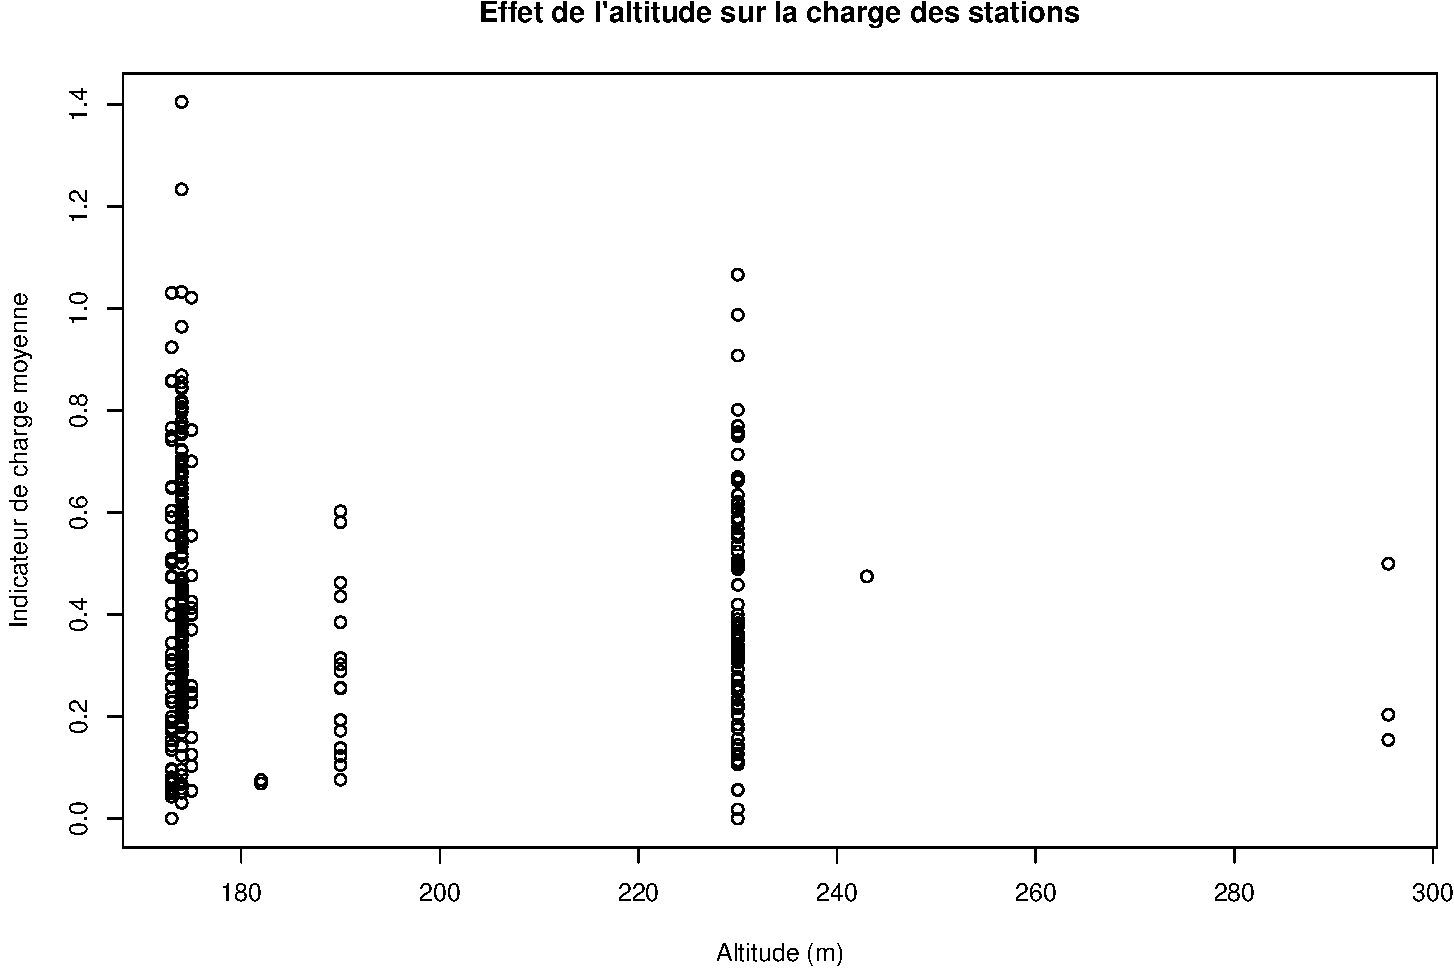
\includegraphics{Seance7_files/figure-beamer/unnamed-chunk-13-1.pdf}

\end{frame}

\begin{frame}{Aspect ratio, 45°}
\protect\hypertarget{aspect-ratio-45}{}

Heuristic: use the aspect ratio that results in an average line slope of
45°.

Cleveland, William S., Marylyn E. McGill, and Robert McGill. ``The shape
parameter of a two-variable graph.'' Journal of the American Statistical
Association 83.402 (1988): 289-300.

\end{frame}

\begin{frame}[fragile]{Aire + Echelle}
\protect\hypertarget{aire-echelle}{}

\begin{Shaded}
\begin{Highlighting}[]
\KeywordTok{ggplot}\NormalTok{(}\DataTypeTok{data=}\NormalTok{tempstats.df,}\KeywordTok{aes}\NormalTok{(}\DataTypeTok{x=}\NormalTok{time,}\DataTypeTok{y=}\NormalTok{nbbikes))}\OperatorTok{+}\KeywordTok{geom_area}\NormalTok{()}
\end{Highlighting}
\end{Shaded}

\includegraphics{Seance7_files/figure-beamer/unnamed-chunk-14-1.pdf}

\end{frame}

\begin{frame}[fragile]{Changement de point de vue}
\protect\hypertarget{changement-de-point-de-vue}{}

\begin{Shaded}
\begin{Highlighting}[]
\KeywordTok{ggplot}\NormalTok{(}\DataTypeTok{data=}\NormalTok{tempstats.df,}\KeywordTok{aes}\NormalTok{(}\DataTypeTok{x=}\NormalTok{time,}\DataTypeTok{y=}\KeywordTok{max}\NormalTok{(nbbikes)}\OperatorTok{-}\NormalTok{nbbikes))}\OperatorTok{+}
\StringTok{  }\KeywordTok{geom_area}\NormalTok{()}
\end{Highlighting}
\end{Shaded}

\includegraphics{Seance7_files/figure-beamer/unnamed-chunk-15-1.pdf}

\end{frame}

\begin{frame}{}
\protect\hypertarget{section-10}{}

\textless{}spanclass=``green''\textgreater{} 1 variable numérique

en fonction du

{ temps}

{ + catégories}

\end{frame}

\begin{frame}[fragile]{Données Vélib par stations}
\protect\hypertarget{donnuxe9es-vuxe9lib-par-stations}{}

\begin{Shaded}
\begin{Highlighting}[]
\CommentTok{# téléchargement et remise en forme des données}
\NormalTok{url =}\StringTok{ "http://vlsstats.ifsttar.fr/data/spatiotemporalstats_Velib2018.json"}
\NormalTok{data=}\KeywordTok{fromJSON}\NormalTok{(}\DataTypeTok{file=}\NormalTok{url)}
\NormalTok{extract =}\StringTok{ }\ControlFlowTok{function}\NormalTok{(x)\{}
  \KeywordTok{data.frame}\NormalTok{(}\DataTypeTok{id=}\NormalTok{x}\OperatorTok{$}\StringTok{'_id'}\NormalTok{,}
             \DataTypeTok{time=}\NormalTok{ x}\OperatorTok{$}\NormalTok{download_date,}
             \DataTypeTok{nbbikes =}\NormalTok{ x}\OperatorTok{$}\NormalTok{available_bikes )}
\NormalTok{  \}}
\NormalTok{st_tempstats.df=}\KeywordTok{do.call}\NormalTok{(rbind,}\KeywordTok{lapply}\NormalTok{(data,extract))}
\NormalTok{sel =}\StringTok{ }\NormalTok{st_tempstats.df }\OperatorTok\StringTok{ }\KeywordTok{select}\NormalTok{(id) }\OperatorTok\StringTok{ }\KeywordTok{unique}\NormalTok{() }\OperatorTok\StringTok{ }\KeywordTok{sample_n}\NormalTok{(}\DecValTok{8}\NormalTok{) }\OperatorTok\StringTok{ }\KeywordTok{pull}\NormalTok{()}
\CommentTok{# selection de quelques stations}
\NormalTok{st_tempstats_sub.df =}\StringTok{ }\NormalTok{st_tempstats.df }\OperatorTok\StringTok{ }
\StringTok{  }\KeywordTok{filter}\NormalTok{(id }\OperatorTok\StringTok{ }\NormalTok{sel)}
\end{Highlighting}
\end{Shaded}

\end{frame}

\begin{frame}[fragile]{Line charts superposés}
\protect\hypertarget{line-charts-superposuxe9s}{}

\begin{Shaded}
\begin{Highlighting}[]
\KeywordTok{ggplot}\NormalTok{(}\DataTypeTok{data=}\NormalTok{st_tempstats_sub.df)}\OperatorTok{+}
\StringTok{  }\KeywordTok{geom_line}\NormalTok{(}\KeywordTok{aes}\NormalTok{(}\DataTypeTok{x=}\NormalTok{time,}\DataTypeTok{y=}\NormalTok{nbbikes,}\DataTypeTok{group=}\NormalTok{id,}\DataTypeTok{color=}\KeywordTok{factor}\NormalTok{(id)),}\DataTypeTok{size=}\DecValTok{2}\NormalTok{)}
\end{Highlighting}
\end{Shaded}

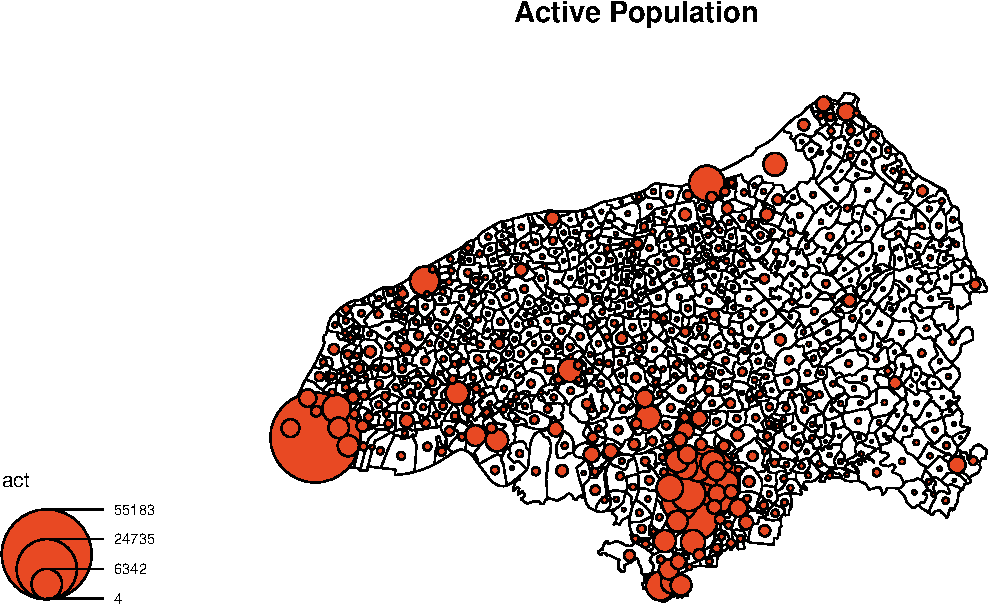
\includegraphics{Seance7_files/figure-beamer/unnamed-chunk-17-1.pdf}

\end{frame}

\begin{frame}[fragile]{Small multiples}
\protect\hypertarget{small-multiples}{}

\begin{Shaded}
\begin{Highlighting}[]
\KeywordTok{ggplot}\NormalTok{(}\DataTypeTok{data=}\NormalTok{st_tempstats_sub.df)}\OperatorTok{+}
\StringTok{  }\KeywordTok{geom_line}\NormalTok{(}\KeywordTok{aes}\NormalTok{(}\DataTypeTok{x=}\NormalTok{time,}\DataTypeTok{y=}\NormalTok{nbbikes,}\DataTypeTok{group=}\NormalTok{id,}\DataTypeTok{color=}\KeywordTok{factor}\NormalTok{(id)),}\DataTypeTok{size=}\DecValTok{2}\NormalTok{)}\OperatorTok{+}
\StringTok{  }\KeywordTok{facet_grid}\NormalTok{(id }\OperatorTok{~}\StringTok{ }\NormalTok{.)}
\end{Highlighting}
\end{Shaded}

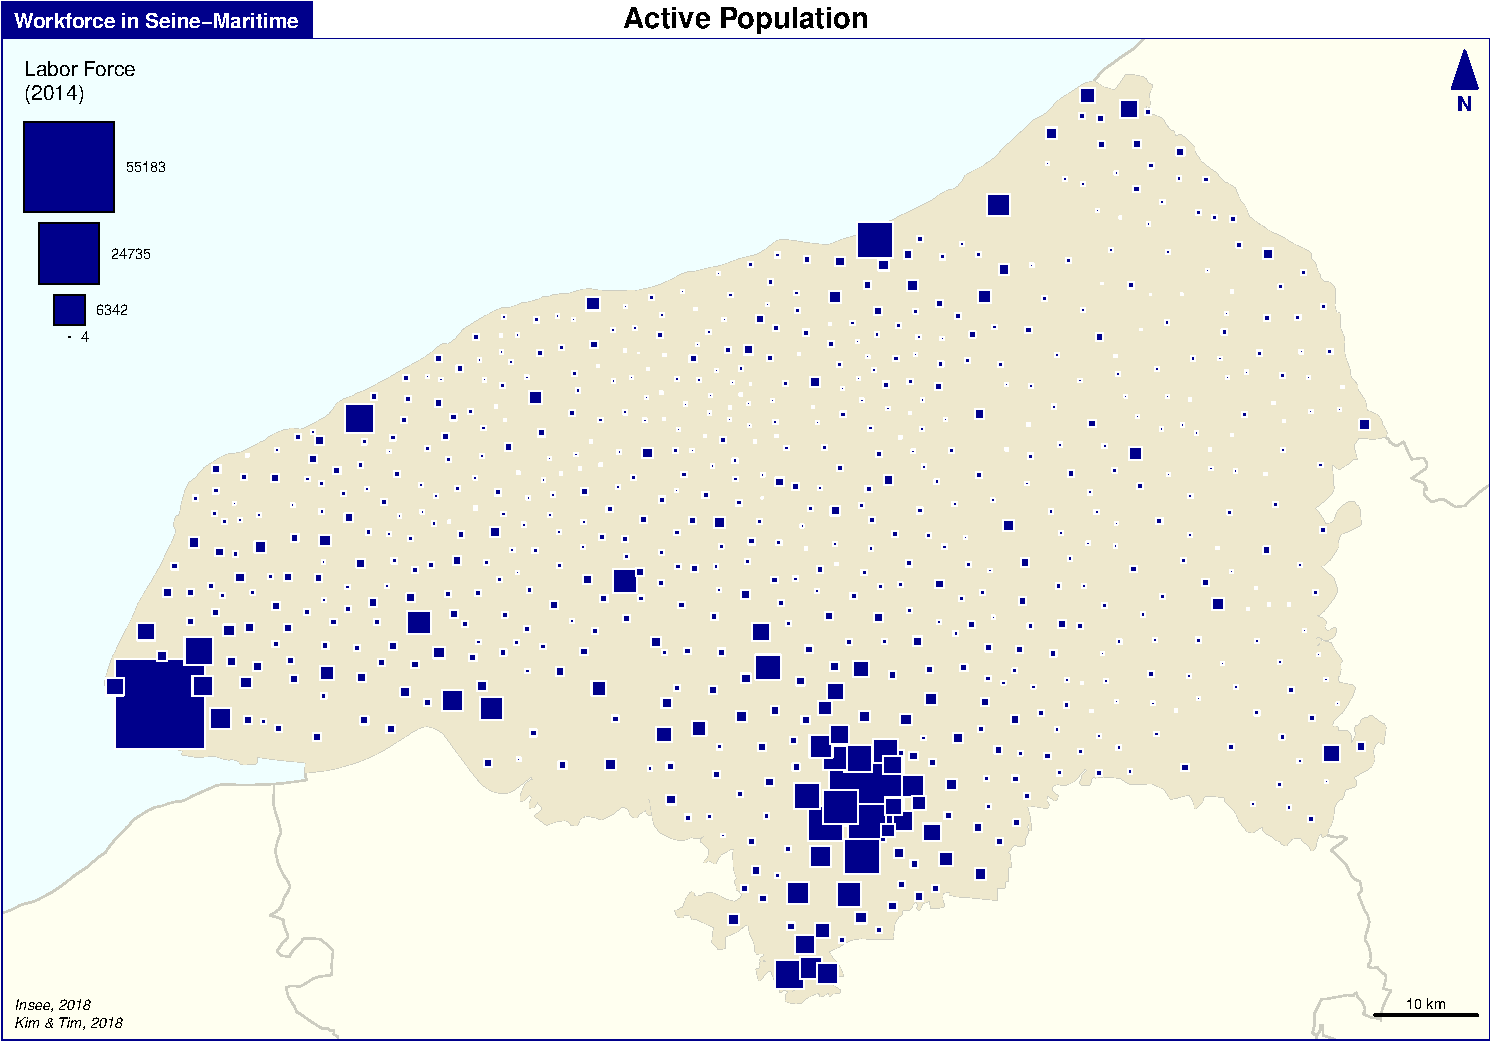
\includegraphics{Seance7_files/figure-beamer/unnamed-chunk-18-1.pdf}

\end{frame}

\begin{frame}{}
\protect\hypertarget{section-11}{}

{ 2 variables numériques}

{ + catégories}

\end{frame}

\begin{frame}[fragile]{Scatter plot + colors}
\protect\hypertarget{scatter-plot-colors}{}

\begin{Shaded}
\begin{Highlighting}[]
\NormalTok{mpg_su =}\StringTok{ }\NormalTok{mpg }\OperatorTok\StringTok{ }
\StringTok{  }\KeywordTok{filter}\NormalTok{(class }\OperatorTok\StringTok{ }\KeywordTok{c}\NormalTok{(}\StringTok{'compact'}\NormalTok{,}\StringTok{'suv'}\NormalTok{,}\StringTok{'pickup'}\NormalTok{,}\StringTok{'minivan'}\NormalTok{)) }
\KeywordTok{ggplot}\NormalTok{(mpg_su)}\OperatorTok{+}\KeywordTok{geom_point}\NormalTok{(}\KeywordTok{aes}\NormalTok{(}\DataTypeTok{x=}\NormalTok{cty,}\DataTypeTok{y=}\NormalTok{hwy,}\DataTypeTok{color=}\NormalTok{class))}
\end{Highlighting}
\end{Shaded}

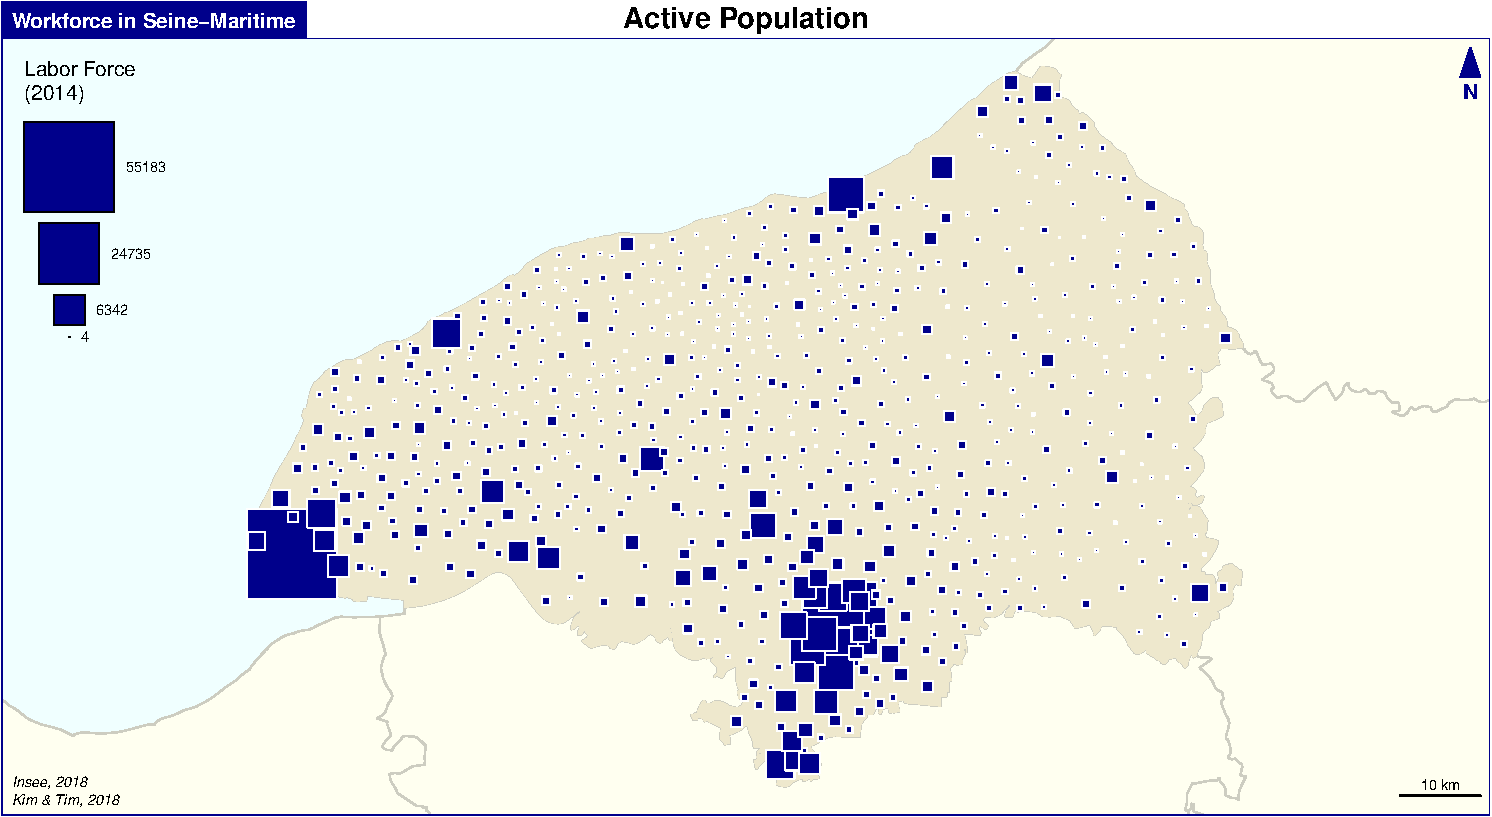
\includegraphics{Seance7_files/figure-beamer/unnamed-chunk-19-1.pdf}

\end{frame}

\begin{frame}[fragile]{Scatter plot + symbols}
\protect\hypertarget{scatter-plot-symbols}{}

\begin{Shaded}
\begin{Highlighting}[]
\NormalTok{mpg_su =}\StringTok{ }\NormalTok{mpg }\OperatorTok\StringTok{ }
\StringTok{  }\KeywordTok{filter}\NormalTok{(class }\OperatorTok\StringTok{ }\KeywordTok{c}\NormalTok{(}\StringTok{'compact'}\NormalTok{,}\StringTok{'suv'}\NormalTok{,}\StringTok{'pickup'}\NormalTok{,}\StringTok{'minivan'}\NormalTok{)) }
\KeywordTok{ggplot}\NormalTok{(mpg_su)}\OperatorTok{+}\KeywordTok{geom_point}\NormalTok{(}\KeywordTok{aes}\NormalTok{(}\DataTypeTok{x=}\NormalTok{cty,}\DataTypeTok{y=}\NormalTok{hwy,}\DataTypeTok{shape=}\NormalTok{class))}
\end{Highlighting}
\end{Shaded}

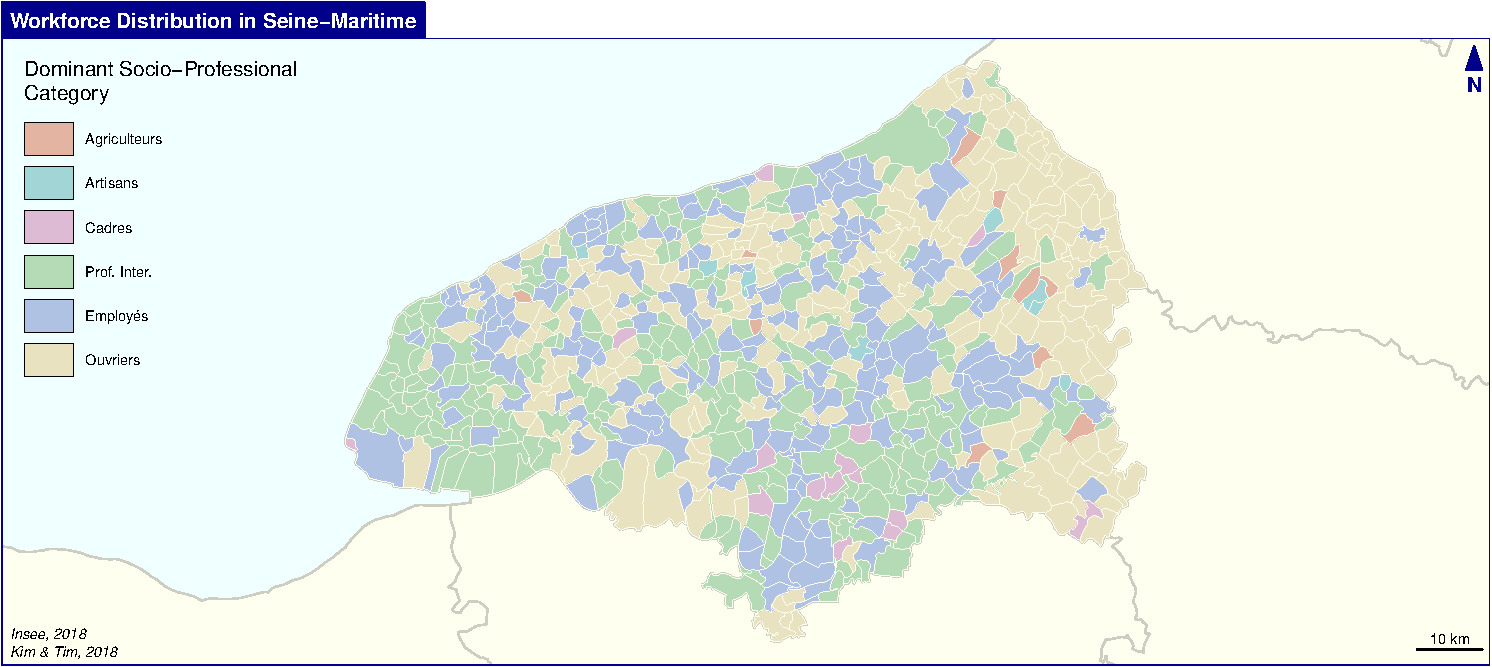
\includegraphics{Seance7_files/figure-beamer/unnamed-chunk-20-1.pdf}

\end{frame}

\begin{frame}{}
\protect\hypertarget{section-12}{}

{ 3 variables numériques (dont une \textgreater{}0)}

{ + catégories}

\end{frame}

\begin{frame}[fragile]{Scatter plot + couleur + taille}
\protect\hypertarget{scatter-plot-couleur-taille}{}

\begin{Shaded}
\begin{Highlighting}[]
\KeywordTok{ggplot}\NormalTok{(mpg_su)}\OperatorTok{+}\KeywordTok{geom_point}\NormalTok{(}\KeywordTok{aes}\NormalTok{(}\DataTypeTok{x=}\NormalTok{cty,}\DataTypeTok{y=}\NormalTok{hwy,}\DataTypeTok{color=}\NormalTok{class,}\DataTypeTok{size=}\NormalTok{displ))}
\end{Highlighting}
\end{Shaded}

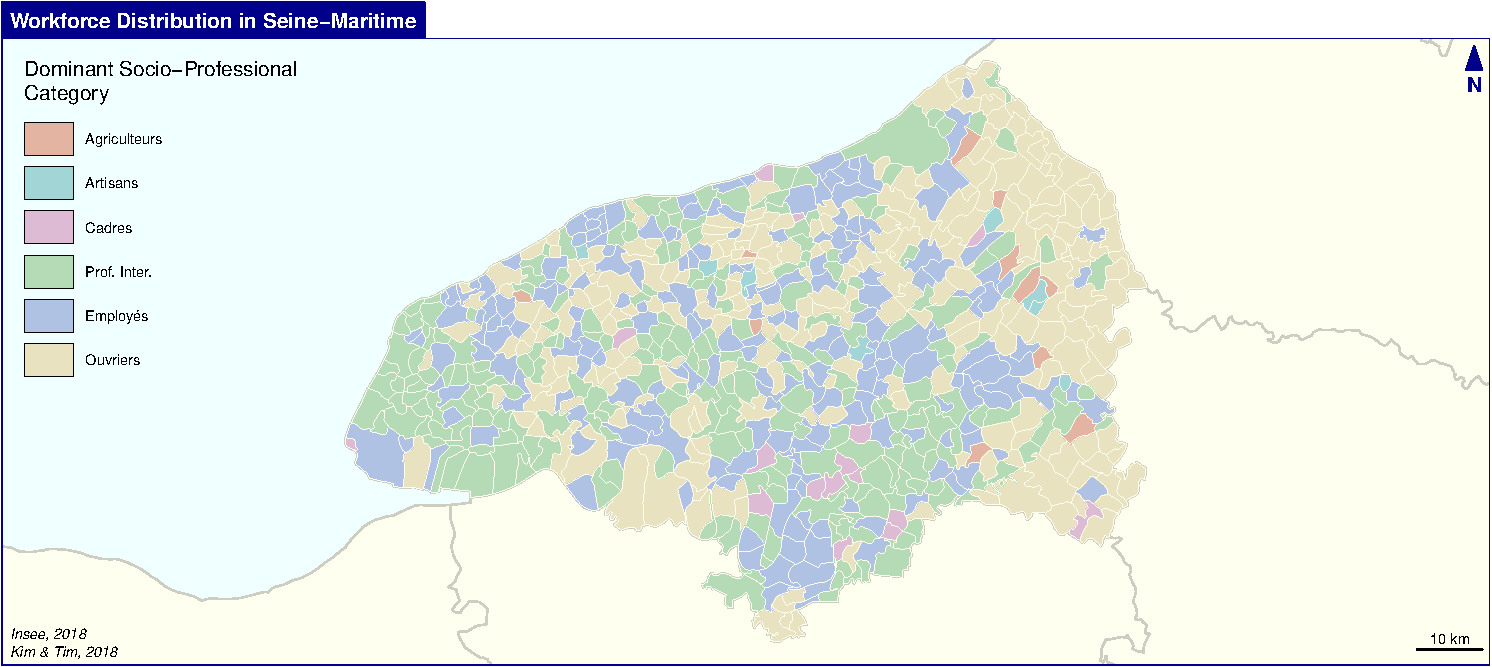
\includegraphics{Seance7_files/figure-beamer/unnamed-chunk-21-1.pdf}

\end{frame}

\begin{frame}[fragile]{Scatter plot + couleur + taille ! echelles}
\protect\hypertarget{scatter-plot-couleur-taille-echelles}{}

\begin{Shaded}
\begin{Highlighting}[]
\KeywordTok{ggplot}\NormalTok{(mpg_su)}\OperatorTok{+}\KeywordTok{geom_point}\NormalTok{(}\KeywordTok{aes}\NormalTok{(}\DataTypeTok{x=}\NormalTok{cty,}\DataTypeTok{y=}\NormalTok{hwy,}\DataTypeTok{color=}\NormalTok{class,}\DataTypeTok{size=}\NormalTok{displ))}
\end{Highlighting}
\end{Shaded}

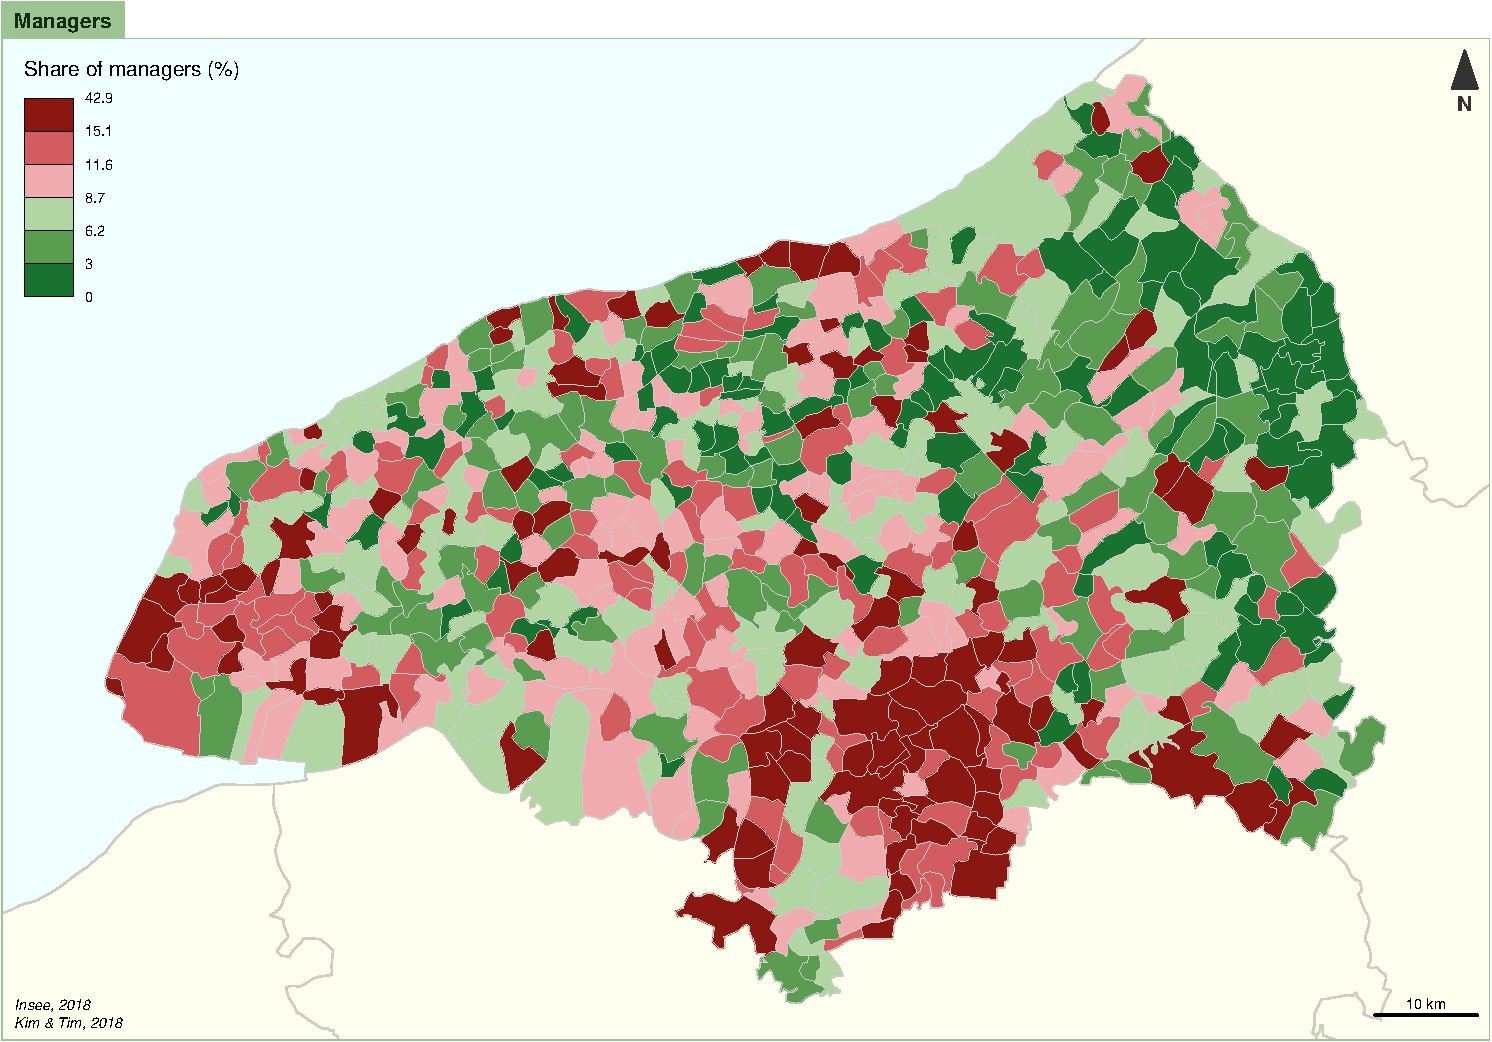
\includegraphics{Seance7_files/figure-beamer/unnamed-chunk-22-1.pdf}

\end{frame}

\begin{frame}{}
\protect\hypertarget{section-13}{}

Taille des cercles : échelle aire ou rayon ?

Rayon

Aire

\end{frame}

\begin{frame}{}
\protect\hypertarget{section-14}{}

\end{frame}

\begin{frame}{}
\protect\hypertarget{section-15}{}

Principes :

Eviter de mentir, Lie Factor

\[\textrm{Lie factor} = \frac{\textrm{visual effect size}}{\textrm{data effect size}}\]

\end{frame}

\begin{frame}{}
\protect\hypertarget{section-16}{}

Lie factor :

\[\textrm{data effect size} = \frac{27.5 - 18}{18} \times 100 = 53 \%\]

Edward Tufte, The Visual Display of Quantitative Information, Cheshire,
CT, Graphics Press, 2001, 2e éd. (1re éd. 1983)

\end{frame}

\begin{frame}{}
\protect\hypertarget{section-17}{}

Lie factor :

\[\textrm{visual effect size} = \frac{5.3 -0.6}{0.6} \times 100 = 783 \%\]

Edward Tufte, The Visual Display of Quantitative Information, Cheshire,
CT, Graphics Press, 2001, 2e éd. (1re éd. 1983)

\end{frame}

\begin{frame}{}
\protect\hypertarget{section-18}{}

Lie factor :

\[\textrm{Lie factor} = \frac{783}{53} = 14.8\]

Edward Tufte, The Visual Display of Quantitative Information, Cheshire,
CT, Graphics Press, 2001, 2e éd. (1re éd. 1983)

\end{frame}

\begin{frame}{}
\protect\hypertarget{section-19}{}

Lie factor : 9.4

Edward Tufte, The Visual Display of Quantitative Information, Cheshire,
CT, Graphics Press, 2001, 2e éd. (1re éd. 1983)

\end{frame}

\begin{frame}{}
\protect\hypertarget{section-20}{}

Sachant que l'aire de la tranche ``apple''" (en vert) est proportionelle
à \(2.22\,cm^2\) et celle correspondant à rim (en bleue) est
proportionelle à \(2.96\,cm^2\) calculer le lying factor ?

\end{frame}

\begin{frame}{Perception}
\protect\hypertarget{perception}{}

\[S = I^p\]

\end{frame}

\begin{frame}{}
\protect\hypertarget{section-21}{}

Principes :

Augmenter la densité de données

\[\textrm{graph data density} = \frac{\textrm{number of entries in data matrix}}{\textrm{area of data display}}\]

\end{frame}

\begin{frame}{}
\protect\hypertarget{section-22}{}

Data density :

Eviter les graphique à faible densité

Edward Tufte, The Visual Display of Quantitative Information, Cheshire,
CT, Graphics Press, 2001, 2e éd. (1re éd. 1983)

\end{frame}

\begin{frame}{}
\protect\hypertarget{section-23}{}

Data density :

Meilleure densité de donnée

Edward Tufte, The Visual Display of Quantitative Information, Cheshire,
CT, Graphics Press, 2001, 2e éd. (1re éd. 1983)

\#\#{Bonnes pratiques :}

éviter de mentir !

faire des graphiques riches

avec des encodages adaptés

de bonnes échelles, (!couleurs, !aires)

des axes labelisés

ordre des facteurs

aspect ratio

format d'enregistrements pdf, svg // png,jpg

\end{frame}

\begin{frame}{{ggplot}}
\protect\hypertarget{ggplot}{}

gg = { grammar of graphics }

``The Grammar of Graphics'' (Wilkinson, Annand and Grossman, 2005)

grammaire → même type de description pour des graphique différents

\end{frame}

\begin{frame}{ggplot}
\protect\hypertarget{ggplot-1}{}

Composants de la grammaires :

{data and aesthetic mappings}, ex : f(data) → x position, y position,
size, shape, color

{geometric objects}, ex : points, lines, bars, texts

{scales}, ex : f({[}0, 100{]}) → {[}0, 5{]} px

{facet specification}, ex : segmentation des données suivant un ou
plusieurs facteurs

{statistical transformations}, ex : moyenne, comptage, régression

{the coordinate system}.

\end{frame}

\begin{frame}{ggplot}
\protect\hypertarget{ggplot-2}{}

Création d'un graphique :

ajout successif de layers (calques)

définissant un mapping des données vers leurs représentation

(+ optionel) définition de transformations statistique

(+ optionel) définition des échelles

(+ optionel) gestion du thème des titre \ldots{}

! Données toujours sous forme de data.frame bien formatées

\end{frame}

\begin{frame}{{ggplot, géométries}}
\protect\hypertarget{ggplot-guxe9omuxe9tries}{}

Création d'un graphique :

ajout successif de layers (calques)

définissant un mapping des données vers leurs représentation

Exemple

\end{frame}

\begin{frame}[fragile]{ggplot}
\protect\hypertarget{ggplot-3}{}

\begin{Shaded}
\begin{Highlighting}[]
\KeywordTok{ggplot}\NormalTok{(mpg,}\KeywordTok{aes}\NormalTok{(}\DataTypeTok{x=}\NormalTok{cty,}\DataTypeTok{y=}\NormalTok{hwy,}\DataTypeTok{color=}\NormalTok{manufacturer))}\OperatorTok{+}\KeywordTok{geom_point}\NormalTok{()}
\end{Highlighting}
\end{Shaded}

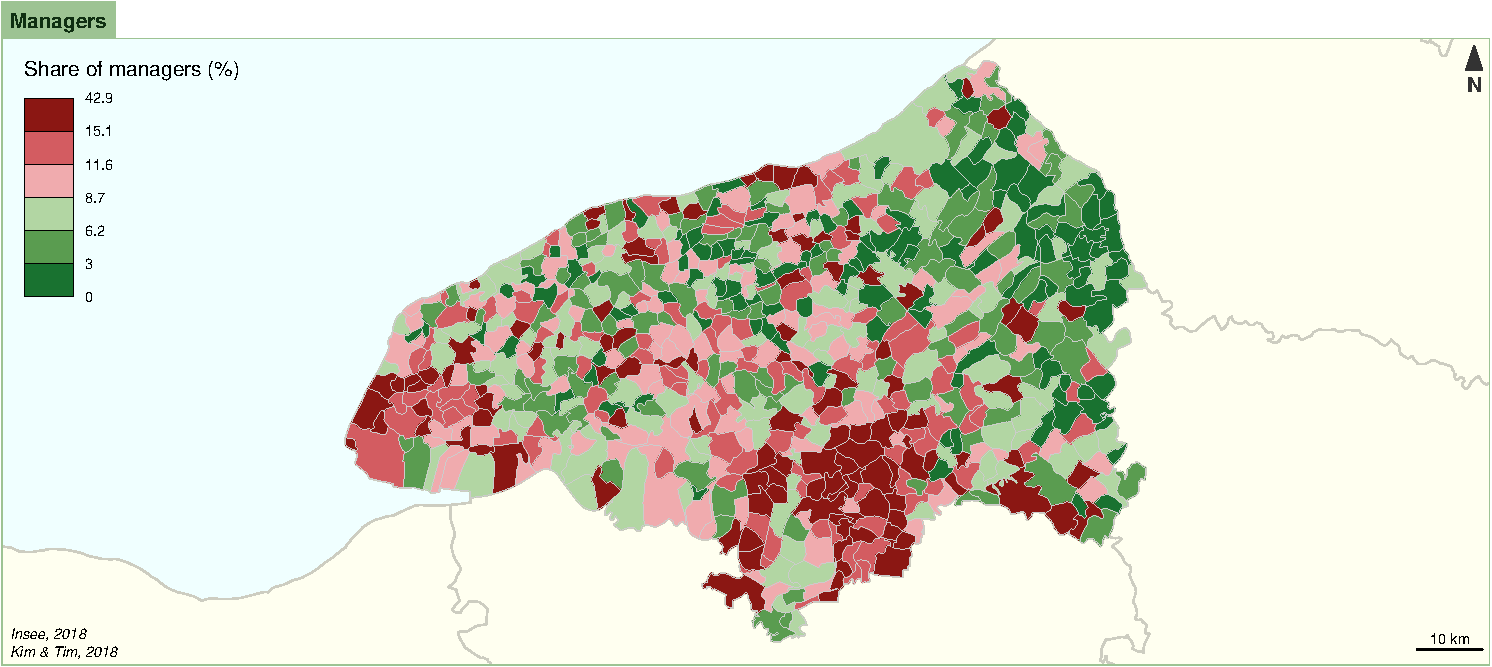
\includegraphics{Seance7_files/figure-beamer/unnamed-chunk-23-1.pdf}

\end{frame}

\begin{frame}[fragile]{ggplot}
\protect\hypertarget{ggplot-4}{}

\begin{Shaded}
\begin{Highlighting}[]
\KeywordTok{ggplot}\NormalTok{(mpg,}\KeywordTok{aes}\NormalTok{(}\DataTypeTok{x=}\NormalTok{cty,}\DataTypeTok{y=}\NormalTok{hwy,}\DataTypeTok{color=}\NormalTok{manufacturer))}\OperatorTok{+}\KeywordTok{geom_jitter}\NormalTok{()}
\end{Highlighting}
\end{Shaded}

\includegraphics{Seance7_files/figure-beamer/unnamed-chunk-24-1.pdf}

\end{frame}

\begin{frame}[fragile]{ggplot}
\protect\hypertarget{ggplot-5}{}

\begin{Shaded}
\begin{Highlighting}[]
\KeywordTok{ggplot}\NormalTok{(mpg,}\KeywordTok{aes}\NormalTok{(}\DataTypeTok{x=}\NormalTok{cty,}\DataTypeTok{fill=}\NormalTok{manufacturer))}\OperatorTok{+}\KeywordTok{geom_histogram}\NormalTok{(}\DataTypeTok{binwidth=}\DecValTok{2}\NormalTok{)}
\end{Highlighting}
\end{Shaded}

\includegraphics{Seance7_files/figure-beamer/unnamed-chunk-25-1.pdf}

\end{frame}

\begin{frame}[fragile]{ggplot}
\protect\hypertarget{ggplot-6}{}

\begin{Shaded}
\begin{Highlighting}[]
\KeywordTok{ggplot}\NormalTok{(mpg,}\KeywordTok{aes}\NormalTok{(}\DataTypeTok{y=}\NormalTok{cty,}\DataTypeTok{x=}\NormalTok{manufacturer))}\OperatorTok{+}\KeywordTok{geom_violin}\NormalTok{()}
\end{Highlighting}
\end{Shaded}

\includegraphics{Seance7_files/figure-beamer/unnamed-chunk-26-1.pdf}

\#\#{ggplot, échelles}

Création d'un graphique :

ajout successif de layers (calques)

définissant un mapping des données vers leurs représentation

en fixant les échelles

\end{frame}

\begin{frame}[fragile]{{ggplot, échelles}}
\protect\hypertarget{ggplot-uxe9chelles}{}

\begin{Shaded}
\begin{Highlighting}[]
\KeywordTok{ggplot}\NormalTok{(mpg,}\KeywordTok{aes}\NormalTok{(}\DataTypeTok{x=}\NormalTok{cty,}\DataTypeTok{y=}\NormalTok{hwy,}\DataTypeTok{color=}\NormalTok{manufacturer,}\DataTypeTok{shape=}\KeywordTok{factor}\NormalTok{(cyl)))}\OperatorTok{+}
\StringTok{  }\KeywordTok{geom_jitter}\NormalTok{()}\OperatorTok{+}
\StringTok{  }\KeywordTok{scale_x_continuous}\NormalTok{(}\DataTypeTok{limits=}\KeywordTok{c}\NormalTok{(}\DecValTok{0}\NormalTok{,}\DecValTok{45}\NormalTok{),}\DataTypeTok{breaks=}\KeywordTok{seq}\NormalTok{(}\DecValTok{0}\NormalTok{,}\DecValTok{45}\NormalTok{,}\DecValTok{2}\NormalTok{))}
\end{Highlighting}
\end{Shaded}

\includegraphics{Seance7_files/figure-beamer/unnamed-chunk-27-1.pdf}

\end{frame}

\begin{frame}{}
\protect\hypertarget{section-24}{}

{Echelles} {de} {couleurs}

\end{frame}

\begin{frame}{Echelle de couleurs}
\protect\hypertarget{echelle-de-couleurs}{}

\url{http://colorbrewer2.org/}

\end{frame}

\begin{frame}{{ggplot, facettes}}
\protect\hypertarget{ggplot-facettes}{}

Création d'un graphique :

ajout successif de layers (calques)

définissant un mapping des données vers leurs représentation

en fixant les échelles

en créant des facettes

\end{frame}

\begin{frame}[fragile]{{ggplot, facettes}}
\protect\hypertarget{ggplot-facettes-1}{}

\begin{Shaded}
\begin{Highlighting}[]
\KeywordTok{ggplot}\NormalTok{(}\DataTypeTok{data=}\NormalTok{mpg,}\KeywordTok{aes}\NormalTok{(}\DataTypeTok{x=}\NormalTok{hwy,}\DataTypeTok{y=}\NormalTok{cty,}\DataTypeTok{color=}\NormalTok{class))}\OperatorTok{+}
\StringTok{  }\KeywordTok{geom_point}\NormalTok{()}\OperatorTok{+}
\StringTok{  }\KeywordTok{facet_wrap}\NormalTok{(}\OperatorTok{~}\NormalTok{year)}
\end{Highlighting}
\end{Shaded}

\includegraphics{Seance7_files/figure-beamer/unnamed-chunk-28-1.pdf}

\end{frame}

\begin{frame}{{ggplot, stats}}
\protect\hypertarget{ggplot-stats}{}

Création d'un graphique :

ajout successif de layers (calques)

définissant un mapping des données vers leurs représentation

en fixant les échelles

en ajoutant des stats

\end{frame}

\begin{frame}[fragile]{ggplot}
\protect\hypertarget{ggplot-7}{}

\begin{Shaded}
\begin{Highlighting}[]
\KeywordTok{ggplot}\NormalTok{(mpg,}\KeywordTok{aes}\NormalTok{(}\DataTypeTok{y=}\NormalTok{cty,}\DataTypeTok{x=}\NormalTok{hwy))}\OperatorTok{+}
\StringTok{  }\KeywordTok{geom_point}\NormalTok{(}\DataTypeTok{color=}\StringTok{"blue"}\NormalTok{)}\OperatorTok{+}\KeywordTok{stat_density2d}\NormalTok{()}
\end{Highlighting}
\end{Shaded}

\includegraphics{Seance7_files/figure-beamer/unnamed-chunk-29-1.pdf}

\end{frame}

\begin{frame}[fragile]{ggplot}
\protect\hypertarget{ggplot-8}{}

\begin{Shaded}
\begin{Highlighting}[]
\KeywordTok{ggplot}\NormalTok{(mpg,}\KeywordTok{aes}\NormalTok{(}\DataTypeTok{y=}\NormalTok{cty,}\DataTypeTok{x=}\NormalTok{hwy))}\OperatorTok{+}
\StringTok{  }\KeywordTok{geom_point}\NormalTok{(}\DataTypeTok{color=}\StringTok{"blue"}\NormalTok{)}\OperatorTok{+}\KeywordTok{stat_smooth}\NormalTok{()}
\end{Highlighting}
\end{Shaded}

\includegraphics{Seance7_files/figure-beamer/unnamed-chunk-30-1.pdf}

\end{frame}

\begin{frame}[fragile]{ggplot}
\protect\hypertarget{ggplot-9}{}

\begin{Shaded}
\begin{Highlighting}[]
\KeywordTok{library}\NormalTok{(hexbin)}
\KeywordTok{ggplot}\NormalTok{(mpg,}\KeywordTok{aes}\NormalTok{(}\DataTypeTok{y=}\NormalTok{cty,}\DataTypeTok{x=}\NormalTok{hwy))}\OperatorTok{+}
\StringTok{  }\KeywordTok{stat_binhex}\NormalTok{()}
\end{Highlighting}
\end{Shaded}

\includegraphics{Seance7_files/figure-beamer/unnamed-chunk-31-1.pdf}

\end{frame}

\begin{frame}[fragile]{Exercices}
\protect\hypertarget{exercices}{}

Reprendre les échelles, légendes de cette figures

\begin{Shaded}
\begin{Highlighting}[]
\CommentTok{# téléchargement et remise en forme des données}
\NormalTok{url=}\StringTok{"http://vlsstats.ifsttar.fr/data/spatiotemporalstats_Velib2018.json"}
\NormalTok{data=}\KeywordTok{fromJSON}\NormalTok{(}\DataTypeTok{file=}\NormalTok{url)}
\NormalTok{extract =}\StringTok{ }\ControlFlowTok{function}\NormalTok{(x)\{}
  \KeywordTok{data.frame}\NormalTok{(}\DataTypeTok{id=}\NormalTok{x}\OperatorTok{$}\StringTok{'_id'}\NormalTok{,}
             \DataTypeTok{time=}\NormalTok{ x}\OperatorTok{$}\NormalTok{download_date,}
             \DataTypeTok{nbbikes =}\NormalTok{ x}\OperatorTok{$}\NormalTok{available_bikes )}
\NormalTok{  \}}
\NormalTok{st_tempstats.df=}\KeywordTok{do.call}\NormalTok{(rbind,}\KeywordTok{lapply}\NormalTok{(data,extract))}
\CommentTok{# selection de 3 stations}
\NormalTok{st_tempstats_sub.df =}\StringTok{ }\NormalTok{st_tempstats.df }\OperatorTok\StringTok{ }
\StringTok{  }\KeywordTok{filter}\NormalTok{(id }\OperatorTok\StringTok{ }\NormalTok{sel)}
\KeywordTok{ggplot}\NormalTok{(}\DataTypeTok{data=}\NormalTok{st_tempstats_sub.df)}\OperatorTok{+}
\StringTok{  }\KeywordTok{geom_line}\NormalTok{(}\KeywordTok{aes}\NormalTok{(}\DataTypeTok{x=}\NormalTok{time,}\DataTypeTok{y=}\NormalTok{nbbikes,}\DataTypeTok{group=}\NormalTok{id,}\DataTypeTok{color=}\KeywordTok{factor}\NormalTok{(id)),}\DataTypeTok{size=}\DecValTok{2}\NormalTok{)}\OperatorTok{+}
\StringTok{  }\KeywordTok{facet_grid}\NormalTok{(id }\OperatorTok{~}\StringTok{ }\NormalTok{.)}
\end{Highlighting}
\end{Shaded}

\end{frame}

\begin{frame}{Exercices}
\protect\hypertarget{exercices-1}{}

Reprendre les échelles, légendes de cette figures
\includegraphics{Seance7_files/figure-beamer/unnamed-chunk-33-1.pdf}

\end{frame}

\begin{frame}{Exercices}
\protect\hypertarget{exercices-2}{}

Reproduire ce graphique (Les données Iris sont déjà chargées)
\includegraphics{Seance7_files/figure-beamer/unnamed-chunk-34-1.pdf}

\end{frame}

\begin{frame}{Exercices}
\protect\hypertarget{exercices-3}{}

Reproduire ce graphique (Les données mtcars sont déjà chargées) !
modifier le theme du graphique ?theme
\includegraphics{Seance7_files/figure-beamer/unnamed-chunk-35-1.pdf}

\end{frame}

\begin{frame}{Exercices}
\protect\hypertarget{exercices-4}{}

Reproduire ce graphique
\includegraphics{Seance7_files/figure-beamer/unnamed-chunk-36-1.pdf}

\end{frame}

\begin{frame}{Exercices}
\protect\hypertarget{exercices-5}{}

Reproduire ce graphique Informations supplémentaires :

Données Vélib de New York

Calculer le taux de remplissage / max(velos disponnibles)

passer en format large

k-means en 8 classes Matrixe X (lignes = stations, colonnes = pas de
temps)

facet + courbes moyennes + transparence (alpha)

\end{frame}

\begin{frame}{Sources}
\protect\hypertarget{sources}{}

\url{https://www.r-graph-gallery.com/index.html}

\url{http://www.cis.umassd.edu/~dkoop/cis467}

\url{https://www.namwkim.org/datavis}

\url{https://courses.cs.washington.edu/courses/cse512}

\url{https://serialmentor.com/dataviz/}

\url{http://socviz.co/gettingstarted.html}

\end{frame}

\end{document}
